\label{visor uavViewer}

Una estación en tierra o GCS (Ground Control Station) es una estación base donde se recibe la
información generada por un dron y con la que se puede monitorizar y controlar toda la actividad
de estos vehículos. Estas estaciones pueden ser fijas o móviles y permiten al operario que maneje el dron
conocer su estado de una manera simple. Uav-viewer es una estación de tierra para drones. Para este
trabajo se ha focalizado en la visión de los datos generados por Ar.Drone y además permite la teleoperación
del cuadricóptero. 

\begin{figure}[H]
  \centering
  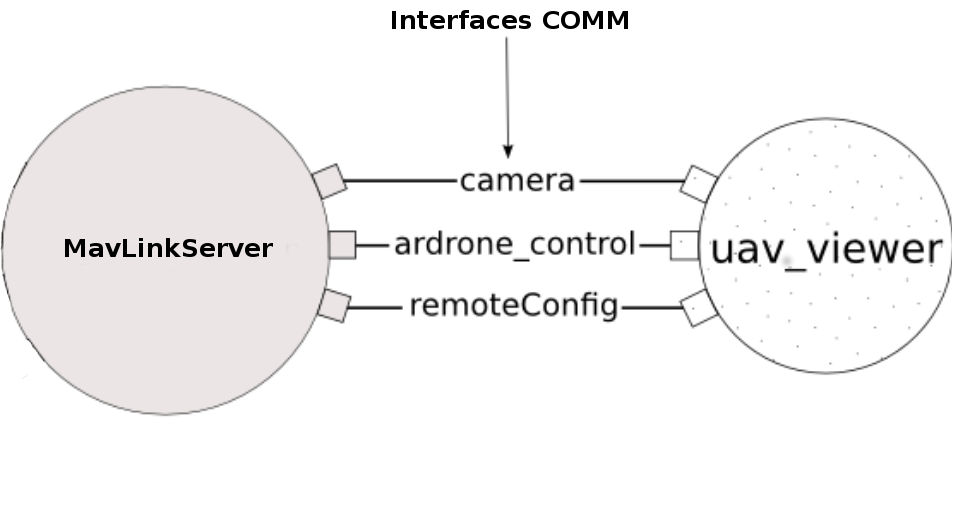
\includegraphics[scale=0.2]{imagenes/Mapageneral.png}
  \caption{Esquema Uav viewer}
  \label{fig:esquemaUav}
\end{figure}

\section{Diseño}

La aplicación ha sido desarrollada en python utilizando para el apartado gráfico la librería
para interfaces de usuario Qt.

En la figura \ref{fig:interfazUavViewer} se muestra la interfaz de este componente.

\begin{figure}[H]
  \centering
  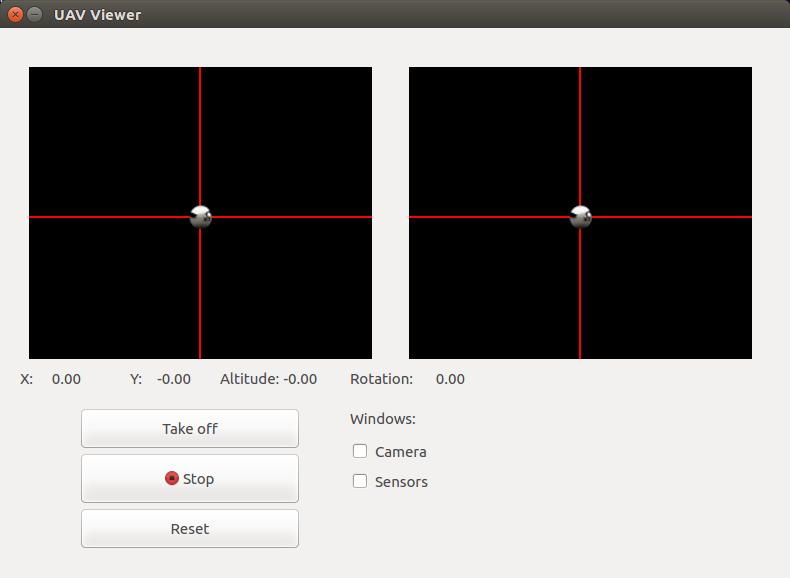
\includegraphics[scale=0.3]{imagenes/Uav_viewer_py.png}
  \caption{Interfaz}
  \label{fig:interfazUavViewer}
\end{figure}

Este interfaz se ha realizado de tal manera que se asemeje lo más posible a los mandos de los drones físicos \ref{fig:mando}. De esta manera desde el joystick izquierdo se controla la altura y el giro (o Yaw) y en el joystick derecho se controlan los ejes X e Y. 

Tambien hay con 3 botones:
\begin{itemize}
\item Take off-Land: sirven para despegar el dron y aterrizar el dron, ese mismo botón cambia el nombre dependiendo el estado del vuelo en el cual nos encontremos
\item Stop: Cuadra los joysticks en la posición (0,0) para detener el dron por completo.
\item Reset: Reinicia los valores por defecto.
\end{itemize}

\begin{figure}[H]
  \centering
  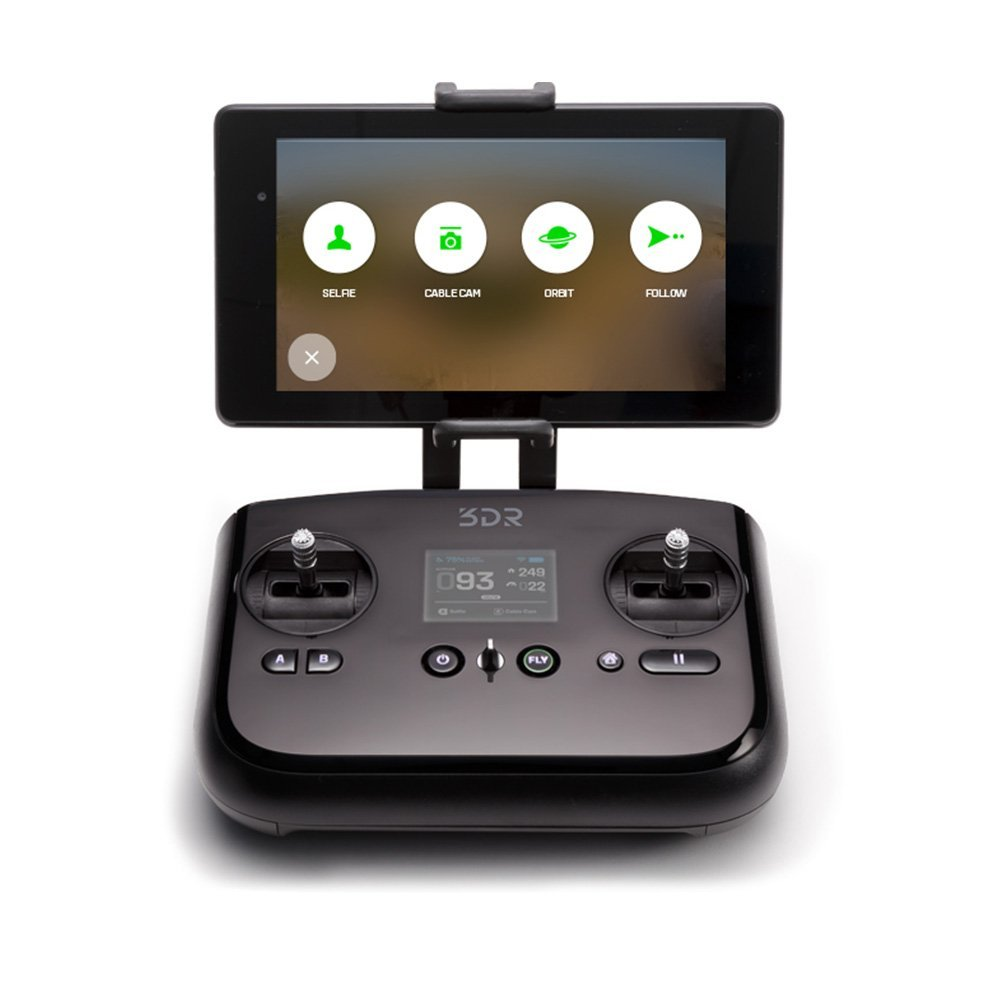
\includegraphics[scale=0.3]{imagenes/mando.jpg}
  \caption{Mando 3dr Solo Dron}
  \label{fig:mando}
\end{figure}

La aplicación tambien implementa de serie 2 utilidades que son la camara y los sensores. Obtiene las imágenes a través de la interfaz camera, para ello se conecta a la interfaz que ofrece el dron. Con la imagen y los metadatos de ésta recuperados desde el dron,
Uav viewer la transforma en una imagen compatible con Qt. En función de la cámara activa, la etiqueta donde se muestran las imágenes cambiará su tamaño para ajustar al ancho y alto de la imagen obtenida. La adquisición de imágenes la realiza la hebra encargada de la comunicación con el dron dentro de un bucle de control independiente a la hebra encargada de la interfaz gráfica. De este modo la hebra encargada de la interfaz gráfica consultará a la hebra que controla el dron periódicamente en busca de nuevas imágenes. Cuando las obtenga, refrescará la imagen que muestra en un determinado periodo de tiempo que puede ser configurado.

\begin{figure}[H]
  \centering
  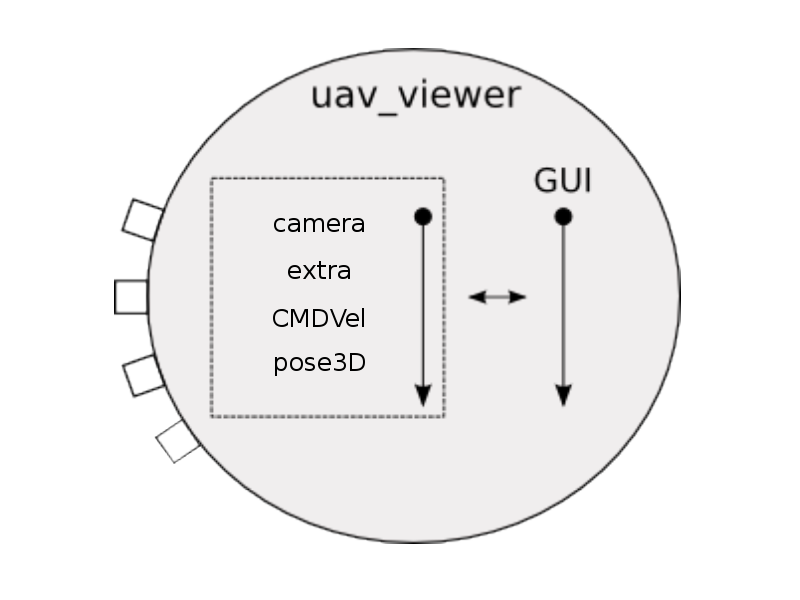
\includegraphics[scale=0.3]{imagenes/uavViewer.png}
  \caption{Hilos Uav Viewer}
  \label{fig:uavViewer}
\end{figure}

Para teleoperar el dron la interfaz gráfica captura los eventos. Estos eventos son creados por los joysticks que enviaran una señal constante con la velocidad indicada para cada unos de los ejes. La interfaz proporcionada por además de ofrecer el envío de
comandos al dron para su control, es capaz de proporcionar los datos de los sensores. A estos datos se los conoce como navdata o datos de navegación. El hilo que comunica Uav viewer con el dron hace uso de ésta interfaz para recibir dichos datos. En la Figura \ref{} se puede apreciar cómo el hilo que gestiona la interfaz de usuario rellena varios objetos gráficos con los datos sensoriales obtenidos del dron. Podemos ver el porcentaje de batería restante, la altitud del dron, con el indicador de actitud podemos visualizar fácilmente el alabeo y el cabeceo, además cuenta con tres velocímetros para indicar la velocidad medida en cada eje. Si esta velocidad es positiva la etiqueta de la velocidad será verde, mientras que si la velocidad es negativa, la etiqueta será roja.
Además de para teleoperar el dron y poder visualizar los datos sensoriales de éste.

\begin{figure}[H]
  \centering
  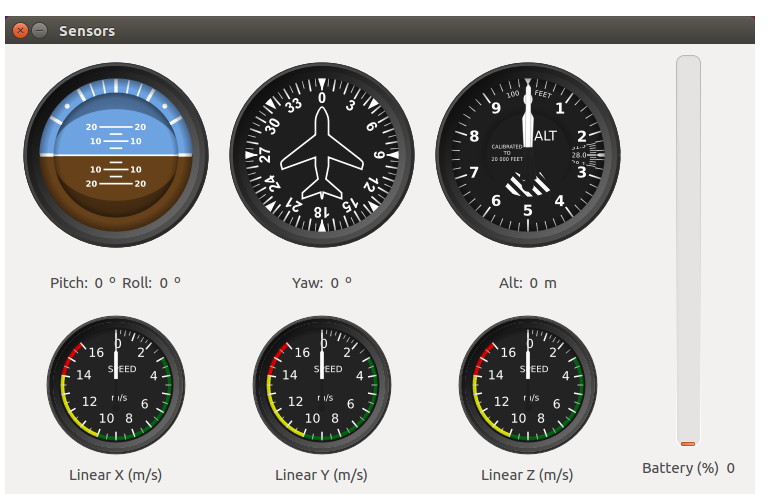
\includegraphics[scale=0.4]{imagenes/sensores.png}
  \caption{Sensores}
  \label{fig:sensores}
\end{figure}

\section{Implementación}

Se utilizan ficheros de configuración YAML, es un formato de serialización de datos legible por humanos inspirado en lenguajes como XML, C, Python, Perl, así como el formato para correos electrónicos especificado por el RFC 2822. YAML fue propuesto por Clark Evans en 2001, quien lo diseñó junto a Ingy döt Net y Oren Ben-Kiki.


{\scriptsize
\begin{verbatim}

UAVViewer:
  Camera: "default -h 0.0.0.0 -p 9995"
  Pose3D: "default -h 0.0.0.0 -p 9996"
  Navdata: "default -h 0.0.0.0 -p 9997"
  CMDVel: "default -h 0.0.0.0 -p 9998"
  Extra: "default -h 0.0.0.0 -p 9999"
\end{verbatim}}

A continuación se muestra el main de la aplicación en el cual iniciaremos la conexión con el interfaz COMM, este interfaz se situa entre nuestra aplicación y tanto los interfaces ICE como los interfaces de ROS. Este nuevo interfaz se ha desarrollado recientemente en JdeRobot como mediador entre las aplicaciones para comunicar indistintamente todos los drivers con la finalidad de abstraer del tipo de comunicación que se realice.

{\scriptsize
\begin{verbatim}
        cfg = config.load(sys.argv[1])

        #starting comm
        jdrc= comm.init(cfg, 'UAVViewer')

        camera = jdrc.getCameraClient("UAVViewer.Camera")
        navdata = jdrc.getNavdataClient("UAVViewer.Navdata")
        pose = jdrc.getPose3dClient("UAVViewer.Pose3D")
        cmdvel = jdrc.getCMDVelClient("UAVViewer.CMDVel")
        extra = jdrc.getArDroneExtraClient("UAVViewer.Extra")

        app = QApplication(sys.argv)
        frame = MainWindow()
        frame.setCamera(camera)
        frame.setNavData(navdata)
        frame.setPose3D(pose)
        frame.setCMDVel(cmdvel)
        frame.setExtra(extra)
        frame.show()



        t2 = ThreadGUI(frame)
        t2.daemon=True
        t2.start()
\end{verbatim}}

Una vez iniciada la aplicación cada componente